%!TEX program = xelatex

\documentclass{xmuthesis}
\graphicspath{{figures/}}            % 图片文件路径
\usepackage{setspace}                % 控制各种间距
\usepackage{ragged2e}                % 主要提供justifying功能,两端对齐
\usepackage{indentfirst}             % 小标题后的第一段默认缩进
\usepackage{amsmath}
\usepackage[super,square,comma]{natbib}    % 引用角标格式
\usepackage{tabularx}                % 表格
\usepackage{float}                   % 清除浮动
\usepackage[section]{placeins}       % 清除浮动
\begin{document}
 %这里引入一个空白符作为第一页是为了使得复制 pdf 的文字不再乱码
\pdfbookmark[0]{封面}{title}          % 封面页加到 pdf 书签
%%设置内容
\title{题目}
\entitle{ Title }
\author{姓名}
\StudentNumber{1234567}
\SchoolName{信息科学与技术学院}
%%\Department{通信工程系}
\Major{通信工程}
\Grade{201x级}
\InnerAdviser{xxx}
\TitleOfInnerAdviser{教授}


\year{二〇1x}
\month{y}
\day{z}

%%封面格式
\thispagestyle{empty}
	
	\begin{center}
		\vspace{25pt}
		
\includegraphics[height=1.8cm]{xmu.png}   
	\end{center}
	
	\begin{spacing}{2.0}
		{\centering{\songti \zihao{-2} \textbf{本\quad 科\quad  毕\quad  业\quad  论\quad  文(论文)}}\\}
		{\centering{{\songti \zihao{-3}(通信工程)} \zihao{3}}\\[1em]}
	\end{spacing}
	
    {\centering{\songti \zihao{2} \textbf{\the\title}}\\}
    \vspace{10pt}
    {\centering{\Roman \zihao{3} \textbf{\the\entitle}}\\}
	\vspace{85pt}
    % \vfill\vfill\vfill
    {\songti\zihao{3}
	 \begin{flushleft}
       \hspace{4em}姓\hspace{2em}名: {\the\author}\\[0.5em]
       \hspace{4em}学\hspace{2em}号: {\the\StudentNumber}\\[0.5em]
       \hspace{4em}学\hspace{2em}院:{\the\SchoolName}\\[0.5em]
       %\hspace{4em}\hspace{3em}系: {\the\Department}\\[0.5em]
       \hspace{4em}专\hspace{2em}业: {\the\Major}\\[0.5em]
	   \hspace{4em}年\hspace{2em}级: {\the\Grade}\\[0.5em]
	   \hspace{4em}指导老师:\makebox[3em]{\the\InnerAdviser}\hspace{4.5em}职称:{\the\TitleOfInnerAdviser}\\[0.5em]
	\end{flushleft}
	\vspace{30pt}
    {\centering{\the\year}年{\the\month}月{\the\day}日 \\}

	}
	\newpage
	\thispagestyle{empty}
	\begin{center}{\songti\zihao{4}\bfseries 厦门大学本科学位论文诚信承诺书}\end{center}
	\par\vspace*{20pt}
	\begin{flushleft}
	\renewcommand{\baselinestretch}{2}
	
	{\justifying{\songti\zihao{4}%
	\hspace{2em}本人呈交的学位论文是在导师指导下独立完成的研究成果。本人在论文写作中参考其他个人或集体已经发表的研究成果,均在文中以适当方式明确标明,并符合相关法律规范及《厦门大学本科毕业论文规范》。\par
	另外,该学位论文为(\hspace{14em})课题(组)的研究成果,获得(\hspace{7.5em})课题(组)经费或实验室的资助,在(\hspace{7.5em})实验室完成。(请在以上括号内填写课题或课题组负责人或实验室名称,未有此项声明内容的,可以不作特别声明。)\par
	\begin{flushright}
	\makebox[24em]{学生声明(签名):\hspace{5em}}\\
	\makebox[16em]{年\hspace{1.5em} 月\hspace{1.5em} 日\hspace{3em}}\\[2em]
	\end{flushright}
	\hspace{2em}该同学呈交的学位论文是在本人指导下独立完成的研究成果。本人已经对学生毕业论文内容进行严格审核,论文写作中参考其他个人或集体已经发表的研究成果,均在文中以适当方式明确标明,并符合相关法律规范及《厦门大学本科毕业论文规范》。\par
	\begin{flushright}
	\makebox[24em]{学生声明(签名):\hspace{5em}}\\
	\makebox[16em]{年\hspace{1.5em} 月\hspace{1.5em} 日\hspace{3em}}\\[2em]
	\end{flushright}
	}}
	\end{flushleft}                % 加入封面

\frontmatter                         % 开始正文之前的部分
\pagenumbering{Roman}                % 正文之前的页码用大写罗马字母编号.

%%%=== 致谢 ===%%%
% !Mode:: "TeX:UTF-8"
% 致谢
\pagestyle{fancy}
     \fancyhf{}
	 \fancyhead{}
	 \chead{\normalfont\small\rmfamily\nouppercase{\leftmark}} 
     \fancyfoot[C]{-\,\thepage\,-}
     \renewcommand{\headrulewidth}{0.4pt}

\begin{acknowledgement}
\begin{center}
		\heiti \zihao{-3}致谢 \\[2em]
	\end{center}
\begin{flushleft}
\hspace{2em}感谢大家!
\end{flushleft}
\end{acknowledgement}               % 致谢
% !Mode:: "TeX:UTF-8"

%%======中文摘要===========================%
\pagestyle{fancy}
     \fancyhf{}
	 \fancyhead[CO]{\normalfont\small\rmfamily\nouppercase{\leftmark}}
     \fancyfoot[C]{-\,\thepage\,-}
     \renewcommand{\headrulewidth}{0.4pt}
     
     
\begin{cnabstract}
\begin{center}
		\heiti \zihao{-3}题目 \\[2em]
	\end{center}
%%\begin{flushleft}
\zihao{-4}\heiti[摘要]\quad 
\songti\zihao{-4}摘要内容
\\[2em]\zihao{-4}\heiti[关键词]\quad 
\songti\zihao{-4}关键词1;关键词2;关键词3\qquad 
%%\end{flushleft}
\end{cnabstract}


%%====英文摘要==========================%
\begin{enabstract}
\begin{center}
		\textsf{\zihao{-3} Title} \\[2em]
\end{center}
\arial{\zihao{-4}[Abstract]\quad
\zihao{-4}content
\\[2em]\zihao{-4}[Keywords]\quad
\zihao{-4}Keyword1;\quad Keywords2;\quad Keywords3\quad}

\end{enabstract}             % 摘要
\pdfbookmark{目录}{toc}
\tableofcontents

\mainmatter                          % 以下是正文
%%%=== 第一章 引言 ===%%%
\chapter{引言}

\section{研究目的}
本文的研究目的是...
\section{研究方法}
\par
本文的研究方法是...
\section{论文结构}
\par
下面介绍论文之后的行文结构:



%%%=== 第二章 背景 ===%%%
\newpage
\chapter{背景}

\section{历史发展}
相关研究的发展历史……
\section{背景知识}
\subsection{知识点一——列表}

\begin{enumerate}
	\item 第一项
	\item 第二项
	\item 第三项
	\item 第四项
\end{enumerate}
\subsection{知识点二——图片}
\begin{center}
	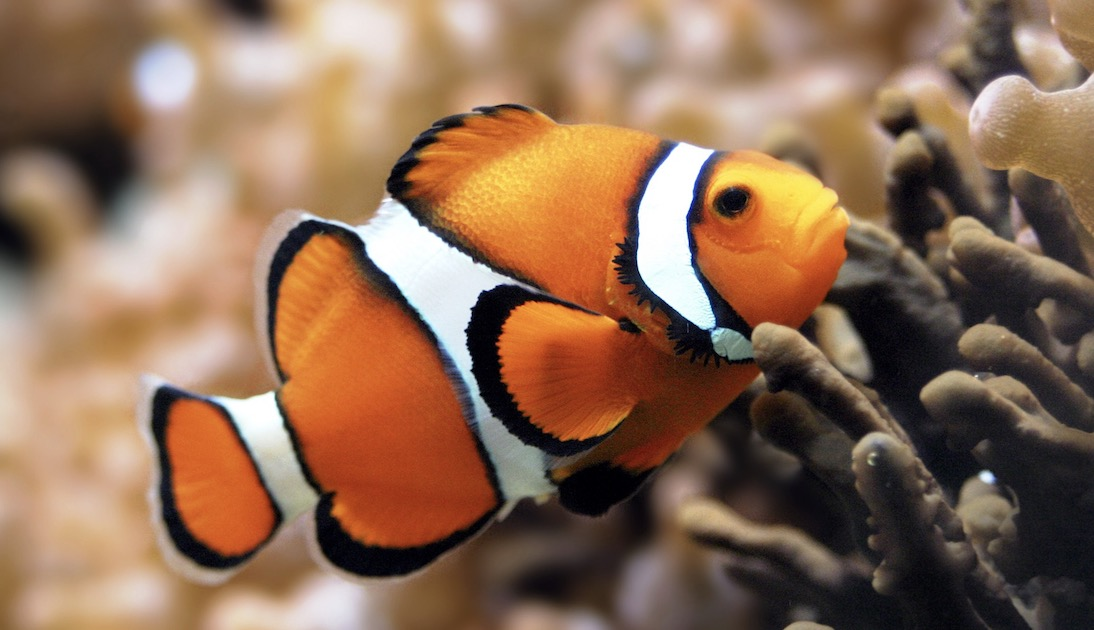
\includegraphics[scale=0.3]{fish.jpg}  \\  
\end{center}
\par
\subsection{清除图片浮动}
\begin{figure}[htb]
  \centering
  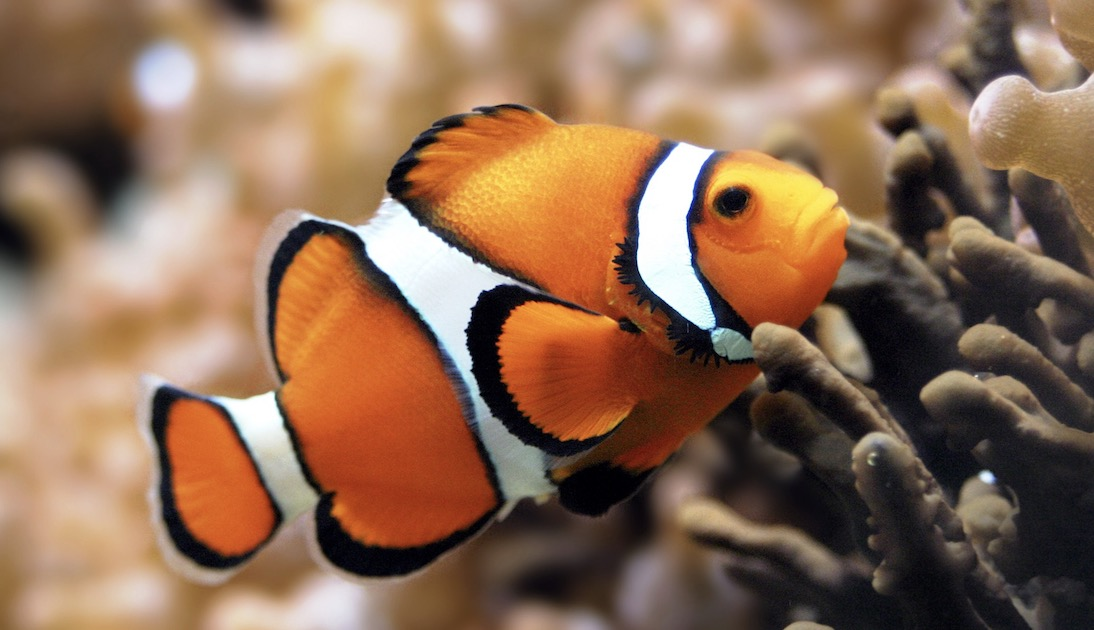
\includegraphics[height=4cm]{fish.jpg}
  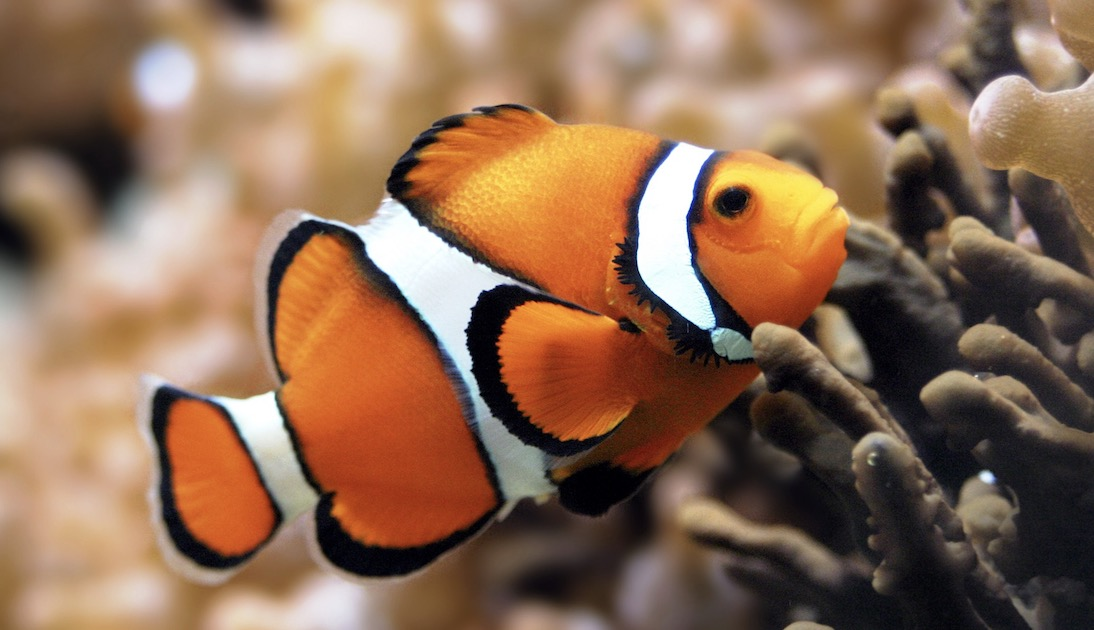
\includegraphics[height=4cm]{fish.jpg}\\
  \caption{Fish}
\end{figure}



















%%%=== 第三章 原理 ===%%%
\newpage
\chapter{原理}

\section{研究方向一}
\subsection{算法原理}
行间公式$G^l \in R^{N_l \times N_l}$
\subsection{实现方法}
公式:
\[
L_{content}(\vec{p},\vec{x},l) = \frac{1}{2}\sum_{i,j}(F^l_{ij} - P^l_{ij})^{2} \tag{1}
\]
公式2:
\[
\frac{\partial{L_{content}}}{\partial{F^l_{ij}}} = 
\begin{cases}
(F^l - P^l)_{ij} & \text{if } {F^l_{ij}} > 0,\\
0 & \text{if } {F^l_{ij}} < 0.
\end{cases} \tag{2}
\]
\par
\section{研究方向二}
\subsection{基本思想}

\subsection{实现方法}
\subsubsection{第一步}

\subsubsection{第二步}

\subsubsection{第三步}















%%%=== 第四章 实验 ===%%%
\newpage
\chapter{实验}

\section{前期准备}

\section{实验步骤}

\section{实验相关参数}
 表格展示:\\
\par
\begin{center}
 \begin{tabularx}{30em}%
{|*{5}{>{\centering\arraybackslash}X|}}
  \hline
  item &  x & y & z & k \\ \hline
  first & 50 & 1 & 25 & 4 \\ \hline
  second & 38 & 1 & 20 & 4 \\ \hline
  third & 40 & 1 & 20 & 4 \\ \hline
  fourth & 42 & 1 & 18 & 4 \\ \hline
\end{tabularx}
\end{center}
\section{其他问题}




%%%=== 第五章 结果 ===%%%
\newpage
\chapter{结果}
\section{实验结果展示}

\section{结果分析}
\subsection{速度}

\subsection{效果}

\subsection{验证}

\section{比较}
\subsection{另一种方法}

\subsection{这种方法}



%%%=== 第六章 总结===%%%
\newpage
\chapter{总结}
本文结论

\backmatter

%%%=== 参考文献 ===%%%
%%===参考文献===%%
\bibliographystyle{abbrv}           % 参考文献样式,plain,unsrt,alpha,abbrv,chinesebst 等等
\clearpage\phantomsection
\addcontentsline{toc}{chapter}{参考文献}
\begin{thebibliography}{00}

  \bibitem{r1} Gatys, L.A., Ecker, A.S., Bethge, M.: A neural algorithm of artistic style [J]. arXiv preprint arXiv:1508.06576, 2015.
  \bibitem{r2} Gatys, L.A., Ecker, A.S., Bethge, M.: Texture synthesis using convolutional neural networks [J]. In: Advances in Neural Information Processing Systems 28, May 2015.

\end{thebibliography}

%%%=== 附录 ===%%%
\appendix

\end{document}
% 